\documentclass[12pt]{article}
\usepackage[utf8]{inputenc}
\usepackage{amsmath, amssymb}
\usepackage{listings}
\usepackage{xcolor}
\usepackage{graphicx}
\usepackage{grffile}
\graphicspath{{figs/}}
\DeclareGraphicsExtensions{.pdf,.png,.jpg,.jpeg}

\title{Deep Learning Class Notes}
\author{Your Name}
\date{\today}

\lstset{
    basicstyle=\ttfamily\small,
    backgroundcolor=\color{lightgray!20},
    frame=single,
    breaklines=true,
    keywordstyle=\color{blue},
    commentstyle=\color{green!70!black},
    stringstyle=\color{red},
    numbers=left,
    numberstyle=\tiny,
    stepnumber=1,
    numbersep=5pt,
    showstringspaces=false
}

\begin{document}

\maketitle

\section{Introducción}

\subsection{Básicos de programación}

Programación orientada a objetos: Encapsulamiento: interfaz pública y privada.
Polimorfismo: Sobreescribir el comportamiento predefinido de operaciones.
Herencia: Crear subclases especialización de sus padres.
Los objetos se implementan mediante clases. Esquema para crear entes abstractos (declaración). La instancia es un objeto de la clase específica. 
Existencia lógica: no asigna espacio de memoria al crearse.


Vemos método \textbf{def $\_\_$call$\_\_$(self)}, luego clases heredadas.

\begin{itemize}
    \item \textbf{$\_\_$init$\_\_$}: Inicializa una nueva instancia de la clase.
    \item \textbf{$\_\_$call$\_\_$}: Permite que el objeto sea llamado como una función.
    \item \textbf{$\_\_$str$\_\_$}: Devuelve una representación legible (string) del objeto.
    \item \textbf{$\_\_$repr$\_\_$}: Devuelve una representación oficial del objeto, útil para depuración.
    \item \textbf{$\_\_$getitem$\_\_$}: Permite acceder a elementos usando corchetes (obj[key]).
    \item \textbf{$\_\_$iter$\_\_$}: Permite que el objeto sea iterable en bucles.
    \item \textbf{$\_\_$setitem$\_\_$}: Permite asignar valores a elementos usando corchetes (obj[key] = value).
    \item \textbf{$\_\_$delitem$\_\_$}: Permite eliminar elementos usando corchetes (del obj[key]).
\end{itemize}


\paragraph{Creación de clase padre.} Ejemplo de método que permite identificar errores de implementación a través de una clase heredada.

\begin{figure}
    \centering
    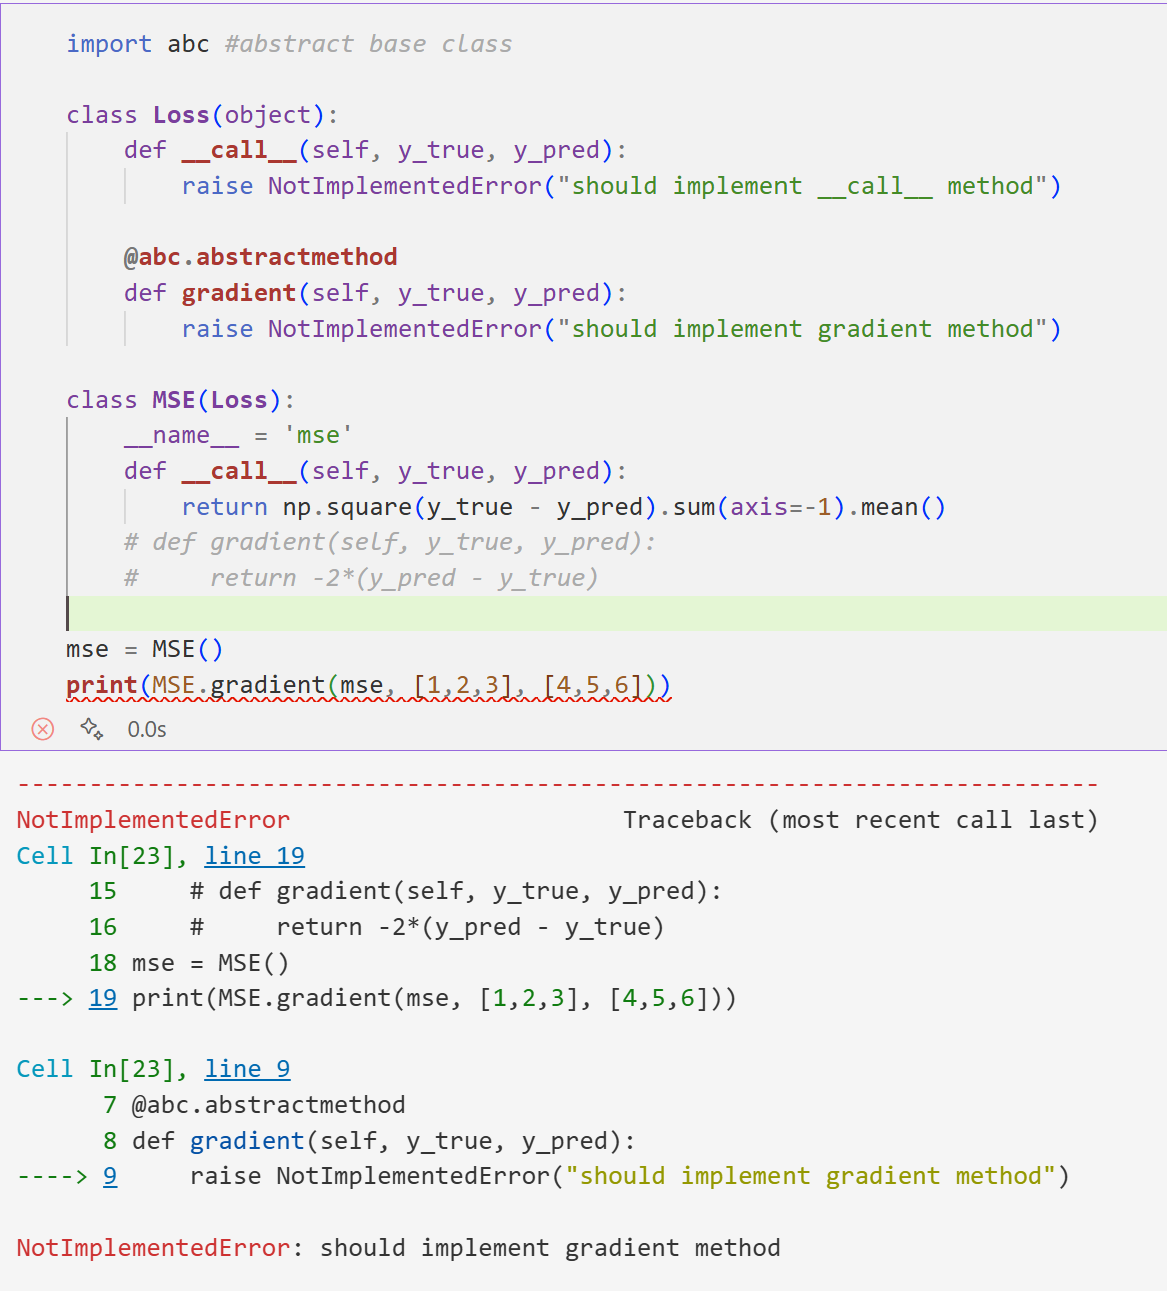
\includegraphics[width=0.5\textwidth]{ejemplo1_abc.png}
\end{figure}

\begin{lstlisting}[language=Python, caption=Simple Neural Network Example]
import torch
import torch.nn as nn

class SimpleNN(nn.Module):
    def __init__(self):
        super(SimpleNN, self).__init__()
        self.fc = nn.Linear(10, 2)
    def forward(self, x):
        return self.fc(x)
\end{lstlisting}

\subsection{Básicos de procesamiento de datos} Funciones de activación. Estudiamos sigmoide, que es la más utilizada históricamente. Necesitamos solucionar el problema de tener valores muy positivos o muy negativos de las entradas. En redes con muchas capas, la regla de la cadena puede llevar al decrecimiento exponencial del gradiente.

Mejor que ReLu: Elu. La derivada es continua cerca de 0. Más costoso compulacionalmente porque computa una exponencial. Swish: producto de lineal con sigmoide. No es plausible con neuronas reales porque la función de activación no puede tener una parte decreciente.


Consenso: ReLU, cuidado con la tasa de aprendizaje porque no satura. Probar Leaky ReLU.


Preprocesamiento de los datos: normalizar y centrar, no tiene sentido para función de activación sigmoide sino tanh. PCA: Considerar 'rotar' y comprimir en términos de varianza en cada coordenada.


Imágenes en color: sustraer la media de cada canal. Imágenes médicas: normalizar cada imagen de manera individual. Tanto para los datos de entrenamiento como para testing.


\paragraph{Inicialización correcta de los pesos:} Si inicio todo en 0, según la función de activación, obtengo resultados diferentes. Propago $0.5$ con sigmoide y $0.0$ con tanh.
$$ a=\sqrt{ \frac{6}{n_{in}+n_{out}} } $$
Inicialización de Glorot: distribución uniforme entre $[-a,a]$
Inicialización de Glorot$\_$normal V2: funciona para RELU


\paragraph{Batch normalization:} Actualización online de las varianzas y las medias.

con $n_{in}, n_{out}$ el número de neuronas a la entrada y salida (parámetro de dimensionalidad de la red)
\end{document}